\newif\ifshowsolutions
\showsolutionstrue
\documentclass{article}
\usepackage{listings}
\usepackage{amsmath}
%\usepackage{subfigure}
% \usepackage{subfig}
\usepackage{amsthm}
\usepackage{amsmath}
\usepackage{amssymb}
\usepackage{graphicx}
\usepackage{mdwlist}
\usepackage[colorlinks=true]{hyperref}
\usepackage{geometry}
\usepackage{titlesec}
\geometry{margin=1in}
\geometry{headheight=2in}
\geometry{top=2in}
\usepackage{palatino}
\usepackage{mathrsfs}
\usepackage{fancyhdr}
\usepackage{paralist}
\usepackage{todonotes}
\setlength{\marginparwidth}{2.15cm}
\usepackage{tikz}
\usetikzlibrary{positioning,shapes,backgrounds}
\usepackage{float} % Place figures where you ACTUALLY want it
\usepackage{comment} % a hack to toggle sections
\usepackage{ifthen}
\usepackage{mdframed}
\usepackage{verbatim}
\usepackage[strings]{underscore}
\usepackage{listings}
\usepackage{bbm}

\usepackage{subcaption}
\usepackage{color}

\rhead{}
\lhead{}

\renewcommand{\baselinestretch}{1.15}

% Shortcuts for commonly used operators
\newcommand{\E}{\mathbb{E}}
\newcommand{\Var}{\operatorname{Var}}
\newcommand{\Cov}{\operatorname{Cov}}
\newcommand{\Bias}{\operatorname{Bias}}
\DeclareMathOperator{\argmin}{arg\,min}
\DeclareMathOperator{\argmax}{arg\,max}

% do not number subsection and below
\setcounter{secnumdepth}{1}

% custom format subsection
\titleformat*{\subsection}{\large\bfseries}

% set up the \question shortcut
\newcounter{question}[section]
\newenvironment{question}[1][]
  {\refstepcounter{question}\par\addvspace{1em}\textbf{Question~\Alph{question}\!
    \ifthenelse{\equal{#1}{}}{}{ [#1 points]}: }}
    {\par\vspace{\baselineskip}}

\newcounter{subquestion}[question]
\newenvironment{subquestion}[1][]
  {\refstepcounter{subquestion}\par\medskip\textbf{\roman{subquestion}.\!
    \ifthenelse{\equal{#1}{}}{}{ [#1 points]:}} }
  {\par\addvspace{\baselineskip}}

\titlespacing\section{0pt}{12pt plus 2pt minus 2pt}{0pt plus 2pt minus 2pt}
\titlespacing\subsection{0pt}{12pt plus 4pt minus 2pt}{0pt plus 2pt minus 2pt}
\titlespacing\subsubsection{0pt}{12pt plus 4pt minus 2pt}{0pt plus 2pt minus 2pt}


\newenvironment{hint}[1][]
  {\begin{em}\textbf{Hint: }}{\end{em}}

\ifshowsolutions
  \newenvironment{solution}[1][]
    {\par\medskip \begin{mdframed}\textbf{Solution~\Alph{question}#1:} \begin{em}}
    {\end{em}\medskip\end{mdframed}\medskip}
  \newenvironment{subsolution}[1][]
    {\par\medskip \begin{mdframed}\textbf{Solution~\Alph{question}#1.\roman{subquestion}:} \begin{em}}
    {\end{em}\medskip\end{mdframed}\medskip}
\else
  \excludecomment{solution}
  \excludecomment{subsolution}
\fi
\newcommand{\boldline}[1]{\underline{\textbf{#1}}}
\usepackage{csquotes}

\setlength{\parskip}{1.2em}

\chead{%
  {\vbox{%
      \vspace{2mm}
      \large
      Machine Learning \& Data Mining \hfill
      Caltech CS/CNS/EE 155 \hfill \\[1pt]
      Miniproject 3\hfill
      Released March $2^{nd}$, 2018 \\
    }
  }
}

\begin{document}
\pagestyle{fancy}

\begin{center}
    \boldline{Late hours used: 2 hour}
\end{center}

\section{Introduction}
\medskip
\begin{itemize}

    \item \boldline{Group members} \\
    Zhewei Chen, Milad Taghavi, Yan Qi Huan
    
    \item \boldline{Team name} \\
    The Magic Marijuana Forest
    
    \item \boldline{Division of labour} \\
    Equal division of work
    
    \item \boldline{Team Code Repository} \\
    https://github.com/miladtaghavi/Miniproject3
    

\end{itemize}

\section{Pre-Processing}

Initially, in the naive HMM we tokenized the dataset by each single words, and for training, the words included in the whole poem chose as the singular sequence. Also the hyphenated words kept as single words to match with the Syllable dictionary. The punctuation is also omitted in pre-processing of the dataset.

For RNN model, in each poem, 40 consecutive characters were grouped as input and the next 10 characters grouped as labels. Here all punctuation kept intact, and the poem numbers are removed. 

In the final model, the last words and the rhyming pair from each poem stored to train the HMM for rhyming. The dataset is also tokenized by single words. All punctuation is also omitted in pre-processing of the dataset expect the punctuation that appears in the hyphenated words. In this model, each singular sequence consists of the sequence of words in each line.

Also since sonnet 99 and 126 do not follow the same format as the rest of the sonnets in dataset, these two sonnets removed from the dataset to assure consistency. 

To further analyze the emission matrices output from the final model(Section 8), the NLTK used to insert the part of speech (POS) on each word of the poems. 


\section{Unsupervised Learning}
% This section should highlight your HMM. What packages did you use, if any? How did you choose the number of hidden states?
For our first model, we simply used the raw words from our preprocessing and trained it using the Hidden Markov Model (HMM) that was used in Homework 6. For simplicity, this model only learns the words and not punctuation or line spacing. The reason for this is that we believed that punctuation would be better learned by using the LSTM model that is described in section 5, while line spacing is constrained by the fact that each line must have 10 syllables in it. 

The package used was the solutions to Homework 6 and we applied the function unsupervised_HMM() from the solution directly. Each input datapoint to the unsupervised HMM is simply a continous list of words from an individual poem, and thus the overall input has 152 entries that each have variable length since each poem has variable length (poems 99 and 126 were excluded due to their different format). The output of the HMM is simply a list of word emissions of any desired length. The number of hidden states was chosen to be 9 as we found that there are 9 general parts of speech in English, namely, noun, verb, adjective, adverb, pronoun, preposition, conjunction, interjection, and article. However, in section 4 below, we also did some systematic testing on the effects of varying the number of hidden states.

\section{Poetry Generation, Part 1: Hidden Markov Models}
% Describe your algorithm for generating the 14-line sonnet. As an example, include at least one sonnet generated from your unsupervised trained HMM. You should comment on the quality of geneating poems in this naive manner. How accurate is the rhyme, rythym, and syllable count, compared to what a sonnet should be? Do your poems make any sense? Do they retain Shakespeare's original voice? How does training with different numbers of hidden states affect the poems generated (in a qualitative manner)? For the good qualities that you describe, also discuss how you think the HMM was able to capture these qualities.
\subsection*{Brief Description of Algorithm}
As briefly described in section 3, each datapoint of input to the HMM is a list of words from each poem with the punctuations and linebreaks stripped. The HMM then runs the unsupervised algorithm that uses the EM algorithm for a fixed number of iterations. Next, it is asked to emit a certain number of words. In our case, we ask it to emit 140 words since we have 14 lines and each line has at most 10 syllables (and thus at most 10 words). Finally, in order to determine the linebreaks, we iterate through the chain of emitted words and break the lines at places where we get 10 syllables (or as close to 10 as possible, since sometimes we have a multisyllabic word at the boundary between 9 and 11 syllabes). The linebreak algorithm is chosen to biased to tiebreak towards a smaller number of syllables if we have a symmetric situation (i.e. it will choose 9 instead of 11 if we have a 2-syllable word at the boundary). Finally, we add commas at the end of each line except the final line where we add a period instead.
\subsection*{Sample Poem}
The following is the raw 140-word emission output from a HMM model with 10 hidden states trained over 50 iterations.

\begin{lstlisting}
the summer it annexed gold doth the used made depends i not stand 
your day will torment when be buds another's great blame hues alone 
let hath of penance thee shall by ignorance grew anticipate whether 
shall have take say smother thy what is live beauty's for all the thee
of on to kind that force as than nourished dead affords give thy heart
nothing up the ambush me thou dost perfection dost me crowned thy 
triumphant love must then from a with which in sweet and may such proof 
marvel even can choose such won least for thou dost is need'st those do 
wilt so still pattern my to yet now thee all which subsist with and hold 
all my done my kind speak fear many mourn is most to my to i on give 
my where and
\end{lstlisting}

We form lines by enforcing the restriction on 10 syllables per line (or closest approximation):


The summer it annexed gold doth the used,

{\parskip=0em 
Made depends I not stand your day will,

Torment when be buds another's great blame,

Hues alone let hath of penance thee shall,

By ignorance grew anticipate whether,

Shall have take say smother thy what is live,

Beauty's for all the thee of on to kind,

That force as than nourished dead affords give,

Thy heart nothing up the ambush me thou,

Dost perfection dost me crowned thy,

Triumphant love must then from a with which,

In sweet and may such proof marvel even,

Can choose such won least for thou dost is need'st,

Those do wilt so still pattern my to yet.
}

\subsection*{Effects of number of hidden states}
In order to determine the number of hidden states that we should use for this HMM, we decided to do experimentation over a wide number of models. Each state was trained for 50 iterations. We print 4 lines of output from each HMM.

\underline{1 hidden state}

{\parskip=0em 
War in with my shall love is I physic,

Thine heart windows plead since that with successive,

Eyes my poor fade concord ride herd my,

Shadow my swift-footed yet thy owner's,}

\underline{2 hidden states}

{\parskip=0em 
They your harsh still aye who I my verse in,

Forests nurseth maiden of not was,

Solemn walls open with being doth a,

More in featureless beauty's acquainted,}

% \underline{5 hidden states}

% {\parskip=0em 
% Must thou but thee their I healthful a with,

% Day cunning since going speak hear thrive then,

% Thee to of engrossed of return my rich,

% Thy when thence my should fear any as be,}

\underline{10 hidden states}

{\parskip=0em 
The summer it annexed gold doth the used,

Made depends I not stand your day will,

Torment when be buds another's great blame,

Hues alone let hath of penance thee shall,}

\underline{25 hidden states}

{\parskip=0em 
Eyes my respose a time's him forbid hath,

Who advocate fair valley-fountain to,

The edge by himself have not or in fool,

Fair question love how fingers knows some of,}

As a qualitative observation, we generally see that with a lower number of hidden states, it is more common to see words that are rarely seen next to one another being placed together, such as ``is I physic'' or ``who I my''. This makes sense because when we have too few states, we do not have sufficient model complexity to sort the words into meaningful categories, leading to words that should have been separate being forced into the same category and thus nonsensical word combinations appearing since we are drawing vastly different words that have been placed into the same bin.

This appears to be somewhat improved in the 10 and 25 hidden states case, although it is still difficult to make a clear-cut judgment. By observation of about 10-20 poems generated, we found that 10 and 25 states produced qualitatively the same poems. Therefore, as mentioned in section 3 above, we decided to use 9 states as there are 9 general parts of speech in English. Therefore, since 9 states showed (from our testing) appeared to be approximately as expressive as 10 and 25 states, we decided on 9 states based on this theoretical justification.

\subsection*{Evaluation}
We first look at some of the good qualities of the poems generated by this first attempt HMM model. Firstly, each line has 9-11 syllables as we enforced this syllable requirement when we split the paragraph of emitted text into separate lines. However, we were unable to ensure that each line has exactly 10 syllables since we could have multisyllabic words appearing on the boundary between below and above 10 syllables. One possible solution could have been to keep regenerating the paragraph of words until we get that all the lines have exactly 10 syllables, but this is potentially time-consuming. A second good quality that we see is that the poems sound somewhat like Shakespeare in terms of phrases that appear in the poem, since the HMM tends to learn word correlations of words that tend to appear adjacent to each other in the original training set.

However, these poems appear to be not particularly coherent in terms of whether each line stands on its own as an individual sentence/clause. The words at the end of each line are often unnatural-sounding, such as ``whether'' and ``will''. This is due to the fact that we learned and emitted text as a single paragraph for the entire poem, and arbitrarily forced each sentence to start a new line once we hit the syllable quota without regard for the contents of that line. We also see that this model fails to predict rhyme in the poem, which is expected since rhyme requires long-range correlations across two lines that inherently cannot be captured in the HMM model which only learns correlations between adjacent words. Both of these issues will be address in section 7 where we build a better multi-stage HMM.

\section{Poetry Generation, Part 2: Recurrent Neural Networks}

We used the implementation of Long Short-Term Memory models (LSTM) in Keras to generate poetry trained on Shakespeare's sonnet character wise. The LSTM took an input of 40 characters and would output the next character in the series, which included newline characters, and thus the LSTM would split the poem into lines on its own. Poetry generation would stop after 14 lines were sampled irregardless of sentence length.

\subsection*{Naive character wise poetry generation}

\noindent Generated Poem at temp =  1.5 :\newline
Seed =  shall i compare thee to a summer's day?

\noindent shall i compare thee to a summer's day? \newline
the simf and day, and parsube a beermer;  \newline
o grast me in waring tand wall if lowe,  \newline
tho ghat the cemplaved white thy praine,  \newline
:secings the herpsto d to thes to be tofleds be ther,  \newline
whan ffor i love farrich you word's se fante,  \newline
lice momh mps mut this my purt cearn thiughtz.  \newline
  knowe in not self ar il besice to sing,  \newline
alt yout to theme wornd so cuncesing theez  \newline
them shaved arivery now,  \newline
hau douth thes my nerezt and you altherzing treen  \newline
cozess mijered she thy erpeode nce rhis hme, \newline
loking grouty cheilt lach oundw things my ming,  \newline
whels offingrest sink oot as thy croult frown? 

\noindent Generated Poem at temp =  0.75 :\newline
Seed =  shall i compare thee to a summer's day?

\noindent shall i compare thee to a summer's day? \newline
thet brouty bind you ast love spreppeace, \newline
but in to in so this dpariing llase (pork, \newline
why shough d ar in thy hade d rice genting? \newline
but no gake clliee notpiris my nempendd. \newline
s miner no hing, and byon thle nempead, \newline
whe chall dey ppire leckine eys bist knepss of my sreemoft daded. \newline
thy fornte azave''s sprace, andize hen fire, \newline
wilt blanty's vence, but dey by mand nr. \newline
  wrrthor thy remightlet may not ent reshith hid  \newline
by pane me non wowt upound, \newline
the vor a coll, nree hos histir grain, \newline
orthit sum of my greckseach sig, my mened \newline
:ut the roth then and ere, \newline
and love's so douts thit thy waint thaight love i laak''s mind, 

\noindent Generated Poem at temp =  0.25 :\newline
Seed =  shall i compare thee to a summer's day?

\noindent shall i compare thee to a summer's day? \newline
thes zifin and fail whith by wey sheet, \newline
then goves do in my prefode thy broudlds, \newline
d aalt should sover, whet beauty's best, \newline
fing the payst risccever i tryee ait, \newline
all blome but merife wouts, \newline
bhat th se fanger thee for my hos ar hail, \newline
farioun the rose whess the the wordd by ank, \newline
and love me anwermeruss dookndss, \newline
f rare her seaver, ozed having toote to ei. \newline
  with latune heart, th tr thy toustel'st food autherp taye, \newline
and that seauty appus wot a timeen softe, \newline
  thin ty that thou toul'zt kerpe me mek, \newline
war ill sinf azt an my beiffand pbride, 

Character wise generation was not successful in generating new words even though LSTM training loss was 0.004 after 100 epochs. Character wise generation had problems generating real words, so we tried constraining to draws to only select characters which will form real words from the sonnet dictionary. The resulting output is shown below.

\subsection*{Poetry generation constraining by real words}

\noindent Generated Poem at temp =  1.5 :\newline
Seed =  shall i compare thee to a summer's day?

\noindent shall i compare thee to a summer's day? \newline
thyself sooner indeed thence surly and pierced:\newline
but merits outstripped tombed thence farther bearer:\newline
but thoughts forth thousand shz loves dost;\newline
matter thyself glowing loves my fell white faring:\newline
late history theez diseased painting lastingz:\newline
but thoughts beauty's sooner that's doom and loves former brainsz\newline
thence thanks wolf issueless ornaments;ignorance vilest reeks\newline
one interest thence tombed tombed thyself transgression surfeit hides\newline
wolf most folly semblance highmost coz\newline
touches thence took:\newline
  sorrows theirs imitated themes wz;celez thez both\newline
and that's borne telling to-themselves reeleth\newline
thee wert ere varying ornaments often owes

\noindent Generated Poem at temp =  0.75 :\newline
Seed =  shall i compare thee to a summer's day?

\noindent shall i compare thee to a summer's day?\newline
these bereft rather under told touches ornaments:\newline
fortune's songs;\newline
and titles often inconstant under something thence forlorn rights former says:\newline
overthrow my jealousy dimmed my head:\newline
thee horses roses bereft seals offenders;\newline
bettered touched therefore youth's ordering stars\newline
:nourished youth's stol'n anticipate muses:\newline
zealous words offenders bereft shallowest\newline
that's sz wolf urge aid they being my defaced.\newline
and doom nothing az now astonished sheaves:\newline
zealous beast seconds oftez swears hastenz languished double-finds\newline
orient my herd spread likeness knit

\noindent Generated Poem at temp =  0.25 :\newline
Seed =  shall i compare thee to a summer's day?

\noindent shall i compare thee to a summer's day?\newline
these bereft read age's thee inward often sighz\newline
thence strength's arts and ashes souls snow\newline
  whence ere pattern abundant others' journey:zealoz trees:\newline
  zealous looks offences dost zealous by thyself\newline
lov'st sheaves strengthened breathz wills\newline
 and injurious air amends\newline
themes if nor fairer history herd;\newline
whence hindmost hot theirs it enclose\newline
windows after-summers':essays yours memory friend.\newline
lour'st once bestow'st towers outstripped;\newline
ashez doom halt theirs ignorance issueless:\newline
indeed thz down-these issueless deeds:\newline
thence horses wombs offenders often something:

The generated poems look better after we constrained the words emitted to only be real words. As expected, the LSTM generated real words because we forced it to. However, the rhythm is still poor and the syllable counts are off. Additionally, the pairs of ending words still do not rhyme. However, the content of the sentences seem somewhat sensible.

We hypothesize that the sonnet structure generation is failing because inputs of 40 characters is not enough to pick up the macro rhyming structure from the previous 2 lines, and 40 characters is only enough to pick up the last line of poetry.

Overall, the LSTM poem quality is still inferior to the HMM we created. Moreover, the runtime for training is longer than HMM as we have a much larger training set by training the model character-by-character instead of word-by-word. This is worsened by the fact that we are training 40-character sequences that are mutually overlapping, which further increases the data size. 

We find that lowering the temperature makes the LSTM recall more exact lines from the sonnets. Conversely, increasing the temperature makes the poetry quality worse since high temperature is like drawing random numbers and taking less information from the LSTM.

% Include generated poems using temperatures of 1.5, 0.75, and 0.25 with the following initial 40-character seed: ``shall i compare thee to a summer’s day\n'', and comment on their differences.


\section{Additional Goals}

% Explore methods of improving your poems or extending them. You do not need to attempt all of the tasks listed in the assignment for full marks on this section. If you have ideas for other improvements to the poetry generation not listed here, feel free to talk to a TA and work on it. The sky is the limit.

\subsection*{Incorporating rhyme, revised syllable counts \& content coherence for HMM}
In this section, we will call the first-attempt HMM model that we developed in sections 4-5 as the \textbf{Naive HMM}  model since we only modelled the poem as a chain of individual words and the linebreaks were only enforced by syllable counts so the lines did not make as much sense on their own. Here, we attempt to improve the quality of HMM poems by implementing 3 new features:
\begin{enumerate}
    \item \textbf{Rhyme}: We first learn which words rhyme and then enforce that the last words of the corresponding lines must rhyme by searching in a dictionary of rhyming words. For each line, we then generate the line backwards by using these last rhyming words as a seed.
    \item \textbf{Syllable counts}: Since we are now generating each line independently instead of generating the entire list of words at once, we can ensure that each line has exactly 10 syllables by regenerating that line if it is mathematically impossible to get exactly 10 syllables.
    \item \textbf{Content coherence}: The previous HMM was a simple Markov chain that only remembers the last word/state and thus did not have any long range correlation between lines that tied content within the poem together. In this model, we introduce a second HMM that specifically learns the last words of each line (skipping past lines that are constrained by rhyme) and thus hopefully it can better capture the overall theme, content or mood of a poem.
\end{enumerate}
\subsubsection*{Brief Description of Algorithm}
There are 3 main steps to this enhanced model. Firstly, we iterate through all the poems excluding 99 and 126 and we extract the words from the corresponding lines that are supposed to rhyme (1 and 3, 2 and 4, ... , 13 and 14). For each pair of rhyming words, we store them into a dictionary and remember which words rhyme with which ones.

Next, we train our first HMM, which we call the ``\textbf{Last-words HMM}''. This model learns the last words of each sonnet from the following line numbers: 1, 2, 5, 6, 9, 10, 13, and thus each poem is a input vector of length 7. The reason for the choices of these line numbers is that the remaining lines are highly constrained by these 7 lines due to the requirement of rhyming, and thus we can consider these 7 lines as ``independent parameters'' that determine the overall content and feel of a poem. We call these 7 lines as ``key lines''. Moreover, by having a large skip (line-by-line as compared to word-by-word from before), we hope to capture more long-range correlations in the text. 

Subsequently, we train our second HMM, which we call the ``\textbf{Reverse-line HMM}''. This HMM reads in each line of a poem in reversed order, so each poem provides 14 datapoints, each with a variable length (number of words in each line). 

We are now ready to generate the poem. Firstly, we use the Last-words HMM to generate the last words for the 7 key lines. Next, we use the rhyming dictionary to find rhyming counterparts to these 7 words and arrange them in the right order (i.e. placing lines 3 and 4 after lines 1,2 etc). Thirdly, we use the Reverse-line HMM with the last words as seeds and generate each line backwards. If the generated line can be cut off at some point to achieve exactly 10 syllables, then we are done. If this is impossible, we then regenerate the line until we get exactly 10 syllables. Finally, we add commas to the end of each line and a period to the last line.

A short note on seeding the HMM is needed here. Since the HMM is only dependent on the previous \textit{state} but not the previous \textit{emission} (word), we need to determine the previous state based on the seed word. This was done by finding the state that had the highest likelihood of generating that seed word, and then seeding that particular state into the HMM.

\subsubsection*{Sample Output from Last-words HMM}
Trained using 9 states and 500 iterations.

\noindent\underline{Emission of 7 last words from lines 1, 2, 5, 6, 9, 10, 13 (key lines)}{\parskip=0pt\par suppose day this created cruel worth bred}

\noindent\underline{Finding rhyming words using the rhyming dictionary for lines 3, 4, 7, 8, 11, 12, 14}{\parskip=0pt\par those stay kiss defeated fuel forth dead}

\noindent\underline{Arranging them in the proper \textit{ababcdcdefefgg} order}{\parskip=0pt\par suppose
day those stay this created kiss defeated cruel worth fuel forth bred dead}

\subsubsection*{Sample Output from Reverse-line HMM}
Trained using 9 states and 200 iterations.


Pleasure did thine being with prove suppose,

{\parskip=0em 
When thy eye of and cheek the the well day,

Better doth and as thou thou in for those,

Hence thought to of shame of your wit and stay,

Compounded return of every find this,

Tongue-tied eye was in lovers for created,

Dress my whom things best mayst be longing kiss,

Strangely despite no the still defeated,

Furrows so or love the truth on his cruel,

Me as one brought thousand fairer my worth,

Or will times but have behold my debt fuel,

Beauty the thy love time's sorrows cold forth,

Thee nor found worship thy abuses bred,

Thee none swift as me every and when dead.
}

\subsubsection*{Evaluation}
This model was the model that we ultimately used for the poem submission. We can immediately see that because we enforced the rhyming structure using the learnt rhyme dictionary, the poem now has the correct \textit{ababcdcdefefgg} rhyme structure: (suppose, those), (day, stay), (this, kiss) etc. Moreover, each line now has exactly 10 syllables instead of approximately 9-11 syllables that we had in the original native HMM model. 

We can also evaluate the effectiveness of the Last-words HMM in providing an overall theme to them poem instead of disparate words. Here are some samples of the last words generated by the Last-words HMM compared to the Naive HMM from section 4:

\textbf{Last-words HMM last words on key lines}
\begin{itemize}
    \item fly foregone spent slave see heart mind
    \item hide mind charged kindness find sadly groan
    \item verse past betray time another you hearts
\end{itemize}

\textbf{Naive HMM last words on key lines}
\begin{itemize}
    \item I frailties gracious far a two should
    \item society suborned with your me gardens love
    \item apple the dead in 'tis thee still
\end{itemize}

While is difficult to judge decisively whether there is a coherent theme within these words, we can see some sort of relation between words that seem reasonable, such as heart \& mind, kindness \& sadly, as well as betray \& hearts. In contrast, the last words of the naive HMM do not appear to have such correlations. Of course, such correlations are certainly subjective also depend on the context of the poem in its entirety. 

Another aspect in which the new model improves over the old naive HMM is that the final words of each line are much more natural-sounding compared to the naive model. This is intuitively understood by the fact that we trained our Last-words HMM on the last words of each poem, so it would definitely prefer these words that appeared in actual poems. In comparison, the last words of the naive model often immediately appear to be unnatural and almost never end a line, such as ``I'', ``'tis'', ``a'', and so on. The line breaks are unnatural since they are simply enforced by syllable constraints. On the flip side, our improved HMM model also potentially suffers from this same problem in the first word of each line, since we cut off each line in the reversed order based on a syllable constraint.

Possible extensions to this model could be done by incorporating rhythm when generating each line from the seed at the end of the sentence. For instance, we could take the training set and assign the stress pattern of each syllable based on the iambic meter of the original poems. We could then use enforce the requirement that we must have syllables with alternating stress patterns when we emit words using the Reverse-line HMM. 

\section{Visualization and Interpretation}

For each of the 9 states in the Reverse-line HMM, we created a word cloud to illustrate the top 10 words in each state based on the transition probability in the emission matrix $O$.

\begin{figure}[H]
	\centering
	\begin{subfigure}[t]{0.3\textwidth}
% 		\centering
		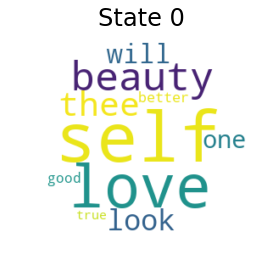
\includegraphics[width=\textwidth]{download(0).png}
		\caption{state 0}
	\end{subfigure}%
	\begin{subfigure}[t]{0.3\textwidth}
% 		\centering
		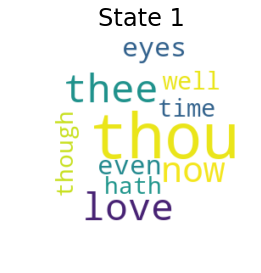
\includegraphics[width=\textwidth]{download(1).png}
		\caption{state 1}
	\end{subfigure}%
	\begin{subfigure}[t]{0.3\textwidth}
% 		\centering
		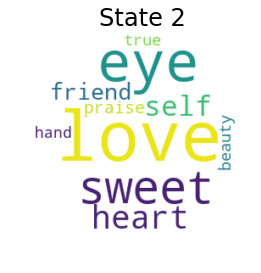
\includegraphics[width=\textwidth]{download(2).png}
		\caption{state 2}
	\end{subfigure}%
	
	\bigskip 
	
	\begin{subfigure}[t]{0.3\textwidth}
% 		\centering
		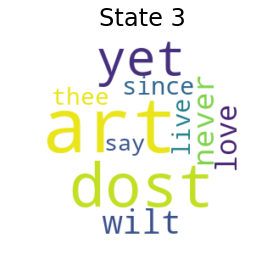
\includegraphics[width=\textwidth]{download(3).png}
		\caption{state 3}
	\end{subfigure}%
	\begin{subfigure}[t]{0.3\textwidth}
% 		\centering
		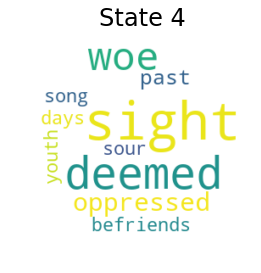
\includegraphics[width=\textwidth]{download(4).png}
		\caption{state 4}
	\end{subfigure}%
	\begin{subfigure}[t]{0.3\textwidth}
% 		\centering
		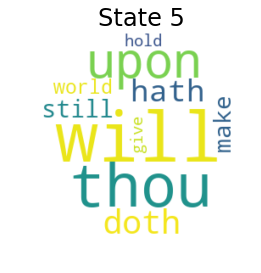
\includegraphics[width=\textwidth]{download(5).png}
		\caption{state 5}
	\end{subfigure}%
	
	\bigskip 
	
	\begin{subfigure}[t]{0.3\textwidth}
% 		\centering
		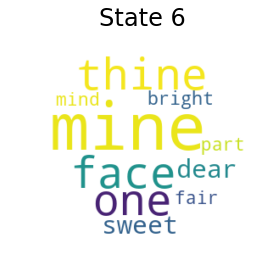
\includegraphics[width=\textwidth]{download(6).png}
		\caption{state 6}
	\end{subfigure}%
	\begin{subfigure}[t]{0.3\textwidth}
% 		\centering
		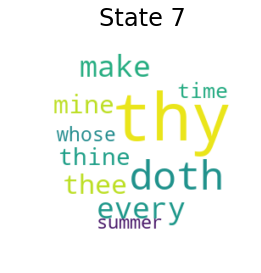
\includegraphics[width=\textwidth]{download(7).png}
		\caption{state 7}
	\end{subfigure}%
	\begin{subfigure}[t]{0.3\textwidth}
% 		\centering
		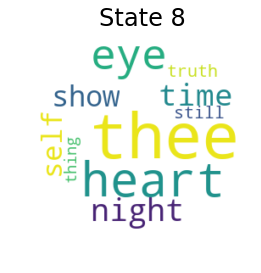
\includegraphics[width=\textwidth]{download(8).png}
		\caption{state 8}
	\end{subfigure}%
	\bigskip 
\end{figure}


In the word cloud, small words such as thy, self, thou, thee, and love tend to dominate. These words have one syllable and tend to rhyme with each other. The same words also shows up in multiple states, meaning Shakespeare's sonnets are formed primarily by a few collection of words which happen to be one syllable in length.

To analyze if the hidden states correlate with parts of speech, we used NLTK to append POS tags to each word and correlated each word/POS with its hidden state via the Viterbi algorithm.

\begin{figure}[H]
	\centering
	\begin{subfigure}[t]{0.3\textwidth}
% 		\centering
		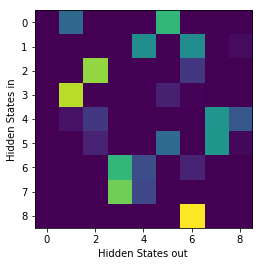
\includegraphics[width=\textwidth]{9x9Transition.png}
		\caption{Transition matrix for 9 hidden states}
	\end{subfigure}%

	\bigskip 

	\begin{subfigure}[t]{0.2\textwidth}
% 		\centering
		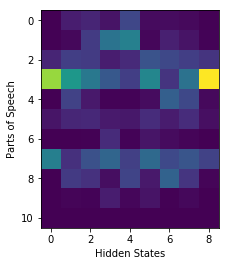
\includegraphics[width=\textwidth]{9states_normalized.png}
		\caption{Normalized frequency of POS}
	\end{subfigure}%
	\begin{subfigure}[t]{0.2\textwidth}
% 		\centering
		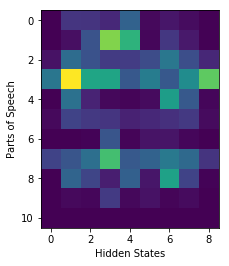
\includegraphics[width=\textwidth]{9state_unnormalized.png}
		\caption{Unnormalized POS frequency for each state}
	\end{subfigure}%
	
\end{figure}

The parts of speech labeled via NLTK \newline
 0) conjunction \newline
 1) interjection \newline
 2) adjective \newline
 3) noun \newline 
 4) pronoun \newline
 5) adverb \newline
 6) preposition \newline
 7) verb \newline
 8) determiner \newline
 9) Miscellaneous 

 The hidden states correlate weakly to the parts of speech. Nouns dominate state 0 and 9. Verb and interjections dominate state 3 and 4. Determiners and pronouns dominate state 6. The parts of speech are somewhat redundant among multiple states, meaning the hidden matrix might be over specified. 
 
Since we saw many words having overlapping states, we decided to decrease the number of total states to 4 to see if we could get better separation between parts of speech and the hidden states.

\begin{figure}[H]
	\centering
	\begin{subfigure}[t]{0.3\textwidth}
% 		\centering
		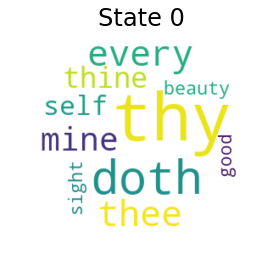
\includegraphics[width=\textwidth]{s1.png}
		\caption{state 0}
	\end{subfigure}%
	\begin{subfigure}[t]{0.3\textwidth}
% 		\centering
		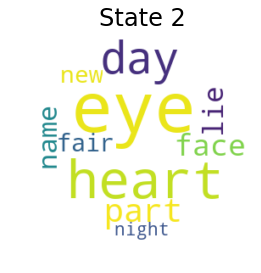
\includegraphics[width=\textwidth]{s3.png}
		\caption{state 1}
	\end{subfigure}%
	
	\bigskip 

	\begin{subfigure}[t]{0.3\textwidth}
% 		\centering
		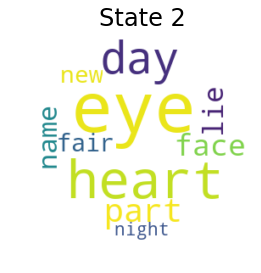
\includegraphics[width=\textwidth]{s3.png}
		\caption{state 2}
	\end{subfigure}%
	\begin{subfigure}[t]{0.3\textwidth}
% 		\centering
		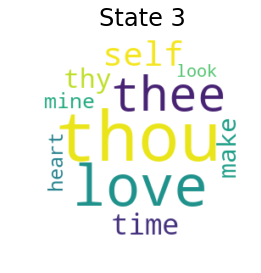
\includegraphics[width=\textwidth]{s4.png}
		\caption{state 3}
	\end{subfigure}%
	
\end{figure}

\begin{figure}[H]
	\centering
	\begin{subfigure}[t]{0.3\textwidth}
% 		\centering
		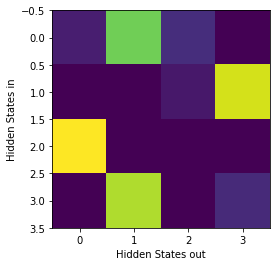
\includegraphics[width=\textwidth]{4x4Transition.png}
		\caption{Transition matrix for 4 hidden states}
	\end{subfigure}%

	\bigskip 

	\begin{subfigure}[t]{0.2\textwidth}
% 		\centering
		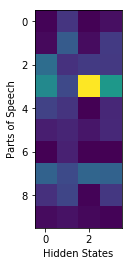
\includegraphics[width=\textwidth]{4states_normalized.png}
		\caption{Normalized frequency of POS}
	\end{subfigure}%
	\begin{subfigure}[t]{0.2\textwidth}
% 		\centering
		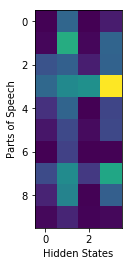
\includegraphics[width=\textwidth]{4state_unnormalized.png}
		\caption{Unnormalized POS frequency for each state}
	\end{subfigure}%
	
\end{figure}

The POS and hidden matrix have the following characteristics: \newline
State 0: Adjectives and nouns tend to show up \newline
State 1: Interjections, determiners, and verbs tend to show up \newline
State 2: Nouns tend to show up \newline
State 3: Nouns and verbs show up  \newline

We see the following interesting transitions: \newline
State 0 from state 1 \newline
State 1 from state 3 \newline
State 2 from state 0 \newline
State 3 from state 1 \newline

Here, we see the output matrix is more sparse, showing distinct transitions between the four states. State 2 appears to be a starting state, meaning it predominately exits the state but wont return. This corresponds with nouns which start the sentence.

This correlates well sentence structure in that nouns are usually next to adjectives and verbs are next to interjections or determiners.

An initial state would likely transition the following way:
2 to 0 to 1 to 3 to 1 to 3 ...

Translated in sentence terms:
Noun to adjectives to verbs to noun to verb to noun ...

This correlates well with english sentence structure, showing how well unsupervised HMM picks up hidden nuances in the english language.

% Explain your interpretation of how a Hidden Markov Model learns patterns in Shakespeare's texts. You should briefly elaborate on the methods you used to analyze the model. In addition, for at least 5 hidden states give a list of the top 10 words that associate with this hidden state and state any common features among these groups. Furthermore, try to interpret and visualize the learned transitions between states. A possible suggestion is to draw a transition diagram of your Markov model and give descriptive names to the states. Feel free to be creative with your visualizations, but remember that accurately representing data is still your primary objective. Your figures, tables, and diagrams should contribute to a discussion about your model.

\end{document}
